% ****** Start of file apssamp.tex ******
%
%   This file is part of the APS files in the REVTeX 4.2 distribution.
%   Version 4.2a of REVTeX, December 2014
%
%   Copyright (c) 2014 The American Physical Society.
%
%   See the REVTeX 4 README file for restrictions and more information.
%
% TeX'ing this file requires that you have AMS-LaTeX 2.0 installed
% as well as the rest of the prerequisites for REVTeX 4.2
%
% See the REVTeX 4 README file
% It also requires running BibTeX. The commands are as follows:
%
%  1)  latex apssamp.tex
%  2)  bibtex apssamp
%  3)  latex apssamp.tex
%  4)  latex apssamp.tex
%
\documentclass[%
 reprint,
%superscriptaddress,
%groupedaddress,
%unsortedaddress,
%runinaddress,
%frontmatterverbose, 
%preprint,
%preprintnumbers,
%nofootinbib,
%nobibnotes,
%bibnotes,
 amsmath,amssymb,
 aps,
%pra,
%prb,
%rmp,
%prstab,
%prstper,
%floatfix,
]{revtex4-2}

\usepackage{graphicx}% Include figure files
\usepackage{dcolumn}% Align table columns on decimal point
\usepackage{bm}% bold math
%\usepackage{hyperref}% add hypertext capabilities
%\usepackage[mathlines]{lineno}% Enable numbering of text and display math
%\linenumbers\relax % Commence numbering lines
\usepackage{enumitem}
\usepackage{tcolorbox}
\usepackage{algorithm}
\usepackage{algpseudocode}

%\usepackage[showframe,%Uncomment any one of the following lines to test 
%%scale=0.7, marginratio={1:1, 2:3}, ignoreall,% default settings
%%text={7in,10in},centering,
%%margin=1.5in,
%%total={6.5in,8.75in}, top=1.2in, left=0.9in, includefoot,
%%height=10in,a5paper,hmargin={3cm,0.8in},
%]{geometry}

\begin{document}

\preprint{APS/123-QED}

\title{Testing an Ornstein--Uhlenbeck Model of Local Field Fluctuations via $T_1$ and $T_2$ Measurements in Pulsed NMR}% Force line breaks with \\


\author{Luca Roncoroni Seda}
\affiliation{University of Southern California, Department of Physics and Astronomy}

\date{May 1, 2026}
    
\begin{abstract}
    We investigate nuclear spin relaxation in liquids using pulsed nuclear magnetic resonance (NMR) and assess the validity of a stochastic dephasing model based on Ornstein-Uhlenbeck (OU) magnetic field fluctuations. Longitudinal and transverse relaxation times, $T_1$ and $T_2$, are measured via inversion recovery and spin-echo experiments using a teaching-scale NMR spectrometer. Assuming isotropic OU noise, these relaxation times are used to extract the correlation time and fluctuation amplitude of the underlying stochastic field. These parameters are then used to simulate stochastic phase accumulation and predict the decay of the spin-echo signal. Comparison between simulation and experiment shows significant deviations for light mineral oil, indicating the presence of other dephasing mechanisms not captured by the isotropic OU model. In contrast, heavy mineral oil exhibits improved agreement when energy relaxation is introduced as a transverse decay mode, indicating that the corresponding dynamics are well-encompassed by the model's assumptions. These results demonstrate that while the OU model provides a useful description of spin dephasing in simple liquids, its applicability is limited in systems with more complicated dynamics. The experiment highlights both the utility and the limitations of stochastic models in describing relaxation phenomena in condensed matter systems.
\end{abstract}

\maketitle

\section{Introduction}
\label{sec:intro}
Pulsed nuclear magnetic resonance (NMR) provides a powerful framework for probing microscopic dynamics through the relaxation of nuclear spin magnetization. Following excitation by a radiofrequency (RF) pulse, the nuclear magnetization evolves toward equilibrium, characterized by two key timescales: the longitudinal and transverse relaxation times $T_1$ and $T_2$, respectively governing the recovery of magnetization along the external field and the loss of phase coherence in the plane normal to it.

While these two time-scales are typically introduced as phenomenological parameters describing exponential relaxation, they may also give insight into the fluctuating nature of molecular-scale magnetic fields. Under a set of assumptions about the sample's equilibrium conditions and local field statistics, we justify the use of an Ornstein--Uhlenbeck (OU) model to describe the behavior of these fluctuating fields.

As a consistency check, we use the measurements of $T_1$ and $T_2$ to extract the relevant parameters of the OU model such as the correlation time and fluctuation amplitude. We then use these parameters to simulate the stochastic phase accumulated between pulses and compare the resulting predicted spin-echo and free-induction decay curves with the experimental signals.

\section{Theoretical Framework}
\label{sec:framework}

\subsection{NMR and spin relaxation}
\label{sec:nmr_relaxation}

Systems whose constituents possess both a magnetic moment and angular momentum exhibit \textit{magnetic resonance} when placed in a strong quasi-static magnetic field. A nucleus with angular momentum $\mathbf{J}=\hbar\mathbf{I}$ and nuclear spin $\mathbf{I}$ has a magnetic moment $\boldsymbol{\mu} = \gamma\mathbf{J}$, where $\gamma$ is called the gyromagnetic ratio. In the presence of an external magnetic field $\mathbf{B}$, the magnetic energy of the nucleus is given by $U = -\boldsymbol{\mu}\cdot\mathbf{B}$. The dipoles $\boldsymbol{\mu}$ tend to align with the strong magnetic field to minimize their energy, so if $\mathbf{B}=B_0 \hat{z}$ we have $U=-\gamma\hbar I_z B_0$.

Spin-$\tfrac{1}{2}$ particles such atomic nuclei have only two allowed values, or states of $I_z$, determined by the magnetic quantum number $m_I = \pm \tfrac{1}{2}$. The energy separation between these states determines the resonant frequency $\omega_0 = \gamma B_0$. In particular, we have
\begin{equation*}
    \Delta U = \hbar \left(\gamma B_0\right) = \hbar\omega_0.
\end{equation*}
The two $m_I$ states are not equally populated; thermal equilibrium favors the lower-energy state according to the Boltzmann distribution. In fact, the net magnetization $\mathbf{M}$ arises from the population difference between spins in the $m_I = +\tfrac{1}{2}$ and $m_I = -\tfrac{1}{2}$ states. In thermal equilibrium, the $x$- and $y$-components of the magnetization average out to zero, while the $z$-component adds up to the total magnetization $M_{z}$.

The sample, however, is not instantly magnetized upon application of the external field. The approach to equilibrium requires both energy and angular momentum exchange between the nuclear spins and their environment (the “lattice”). These processes define the \textit{spin-lattice} relaxation time $T_1$, which governs the exponential recovery of the longitudinal magnetization:
\begin{equation}
    \begin{aligned}
        \frac{dM_z (t)}{dt} &= \frac{M_0 - M_z}{T_1} \\
        \Rightarrow\quad M_z (t) &= M_0 \left(1-e^{-t/T_1}\right),
    \end{aligned}
    \label{eq:T1_recovery}
\end{equation}
where $M_0$ is the equilibrium magnetization, and where we've assumed the initial condition $M_z (0) = 0$.

To generate a net transverse magnetization, the spins must be phase-coherent. In thermal equilibrium, however, the transverse components are randomly oriented, resulting in zero net transverse magnetization. By applying a resonant rotating magnetic field ($\omega = \omega_0$), the magnetization can be coherently driven in the rotating frame $\mathcal{R} = \left(x^*,y^*,z^*\right)$. If the field is turned off after a $\tfrac{\pi}{2}$ pulse--i.e., after a duration such that the magnetization is rotated by $\tfrac{\pi}{2}\,\mathrm{rad}$ in the rotating frame--the magnetization is brought into the $xy$-plane, creating a non-equilibrium transverse magnetization that subsequently precesses about the static field. This magnetization decays exponentially according to the following differential equations:
\begin{align*}
    \frac{dM_{x^*}}{dt} &= -\frac{M_{x^*}}{T_2} \quad\Rightarrow\quad M_{x^*}(t)=M_{x^*0} e^{-t/T_2}\\
    \frac{dM_{y^*}}{dt} &= -\frac{M_{y^*}}{T_2} \quad\Rightarrow\quad M_{y^*}(t)=M_{y^*0} e^{-t/T_2}
\end{align*}

The characteristic decay time $T_2$ is called the \textit{spin-spin} relaxation time, arising from local field fluctuations caused by molecular motion and interactions with neighboring spins. Hence, even if all nuclei begin in phase after the $\tfrac{\pi}{2}$ pulse, they will soon dephase due to these interactions and the net $x$-$y$ magnetization will vanish.

\subsection{Pulsed excitation and measurement}
\label{sec:pnmr}
If we wanted to measure $T_2$, we could simply observe the decay of the transverse magnetization after the $\tfrac{\pi}{2}$ pulse. This curve is called the \textit{free induction decay} (FID). But this method only yields the true $T_2$ if the static field were perfectly uniform. In practice, the spatial inhomogeneities of the static field obscure the part of the decay signal due only to local field fluctuations.

To isolate the intrinsic relaxation time $T_2$, one employs a spin-echo \textit{pulse sequence}, suppressing the dephasing due to the field's inhomogeneities. Starting from equilibrium magnetization $M_0$, a $\tfrac{\pi}{2}$ pulse rotates the magnetization into the transverse plane. The spins then evolve freely for a time $\tau$, during which they dephase due to variations in their local magnetic fields. A subsequent $\pi$ pulse inverts the spin phases about the $x^*$ axis. As a result, spins that had accumulated a phase lead now lag, and vice versa. After an additional time $\tau$, the spins rephase, producing a spin echo at time $2\tau$. For a clear visualization of this process, refer to Figure~\ref{fig:spin-echo-seq}.
\begin{figure*}[!t]
    \centering
    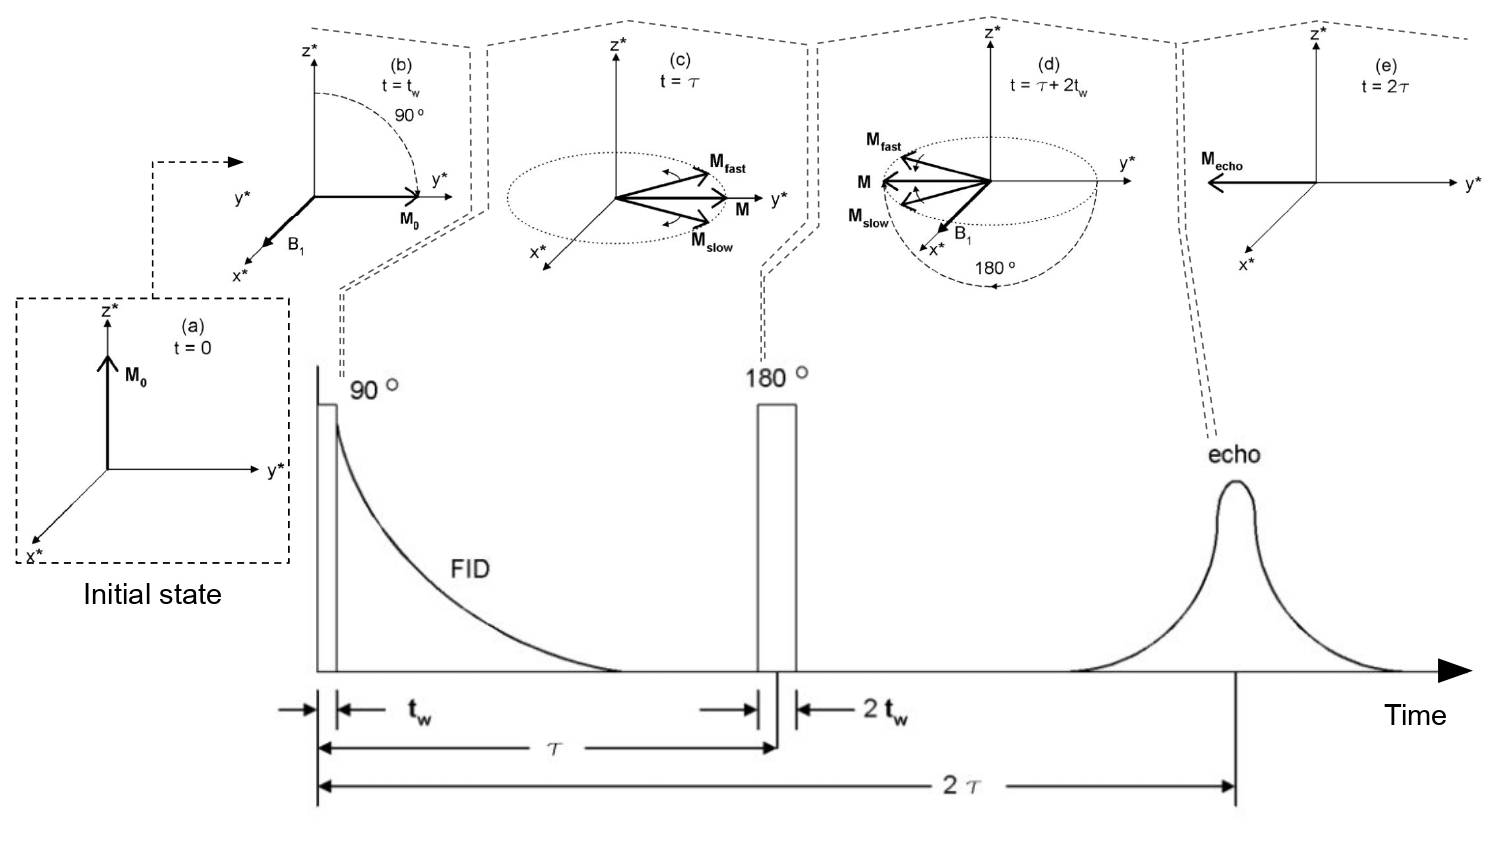
\includegraphics[width=0.8\textwidth]{figures/spin-echo-sequence.jpg}
    \caption{The spin echo pulse sequence, overlaid with the corresponding magnetization response (images courtesy the TeachSpin™ Pulsed/CW NMR student manual). The initial state (a) is rotated 90º by an RF pulse of duration $t_w$ (b). The magnetizations each precess at different rates (slow, medium and fast depicted on the Bloch diagram) depending on the strength of the local field (c), dephasing with a characteristic time set by the FID envelope. After a waiting time $\tau$, all magnetization vectors are rotated by 180º about the $x^*$-axis through an RF pulse of duration $2t_w$, continuing to precess (d). Finally, after a total time $2\tau$, the spins rephase, producing the echo response (e).}
    \label{fig:spin-echo-seq}
\end{figure*}

During this process, however, some transverse magnetization is irreversibly lost due to the stochastic fluctuations of the local magnetic fields at the nuclear sites, which we later model as an Ornstein--Uhlenbeck process. These irreversible processes act throughout the entire evolution time $2\tau$, leading to an exponential decay of the echo amplitude. Accordingly, the transverse magnetization at the echo maximum is given by
\begin{equation}
    M_{xy}(2\tau) = M_0 e^{-2\tau/T_2}.
    \label{eq:T2_recovery}
\end{equation}

The spin-lattice relaxation time $T_1$ can also be recovered by means of a pulse sequence, referred to as inversion recovery. Starting from equilibrium, a $\pi$ pulse is first applied to invert the magnetization, such that $M_z = -M_0$. The system is then allowed to evolve for a variable delay time $\tau$, during which the magnetization relaxes back toward equilibrium due to interactions with the surrounding lattice. After this time, the magnetization is rotated by 90º, and the transverse magnetization decay envelope is observed. Under the initial condition $M_z = -M_0$, Eq.~\ref{eq:T1_recovery} reduces to
\begin{equation}
    M_z(t) = M_0\left(1-2e^{-t/T_1}\right).
    \label{eq:inv-rec-eq}
\end{equation}
\begin{figure*}[!t]
    \centering
    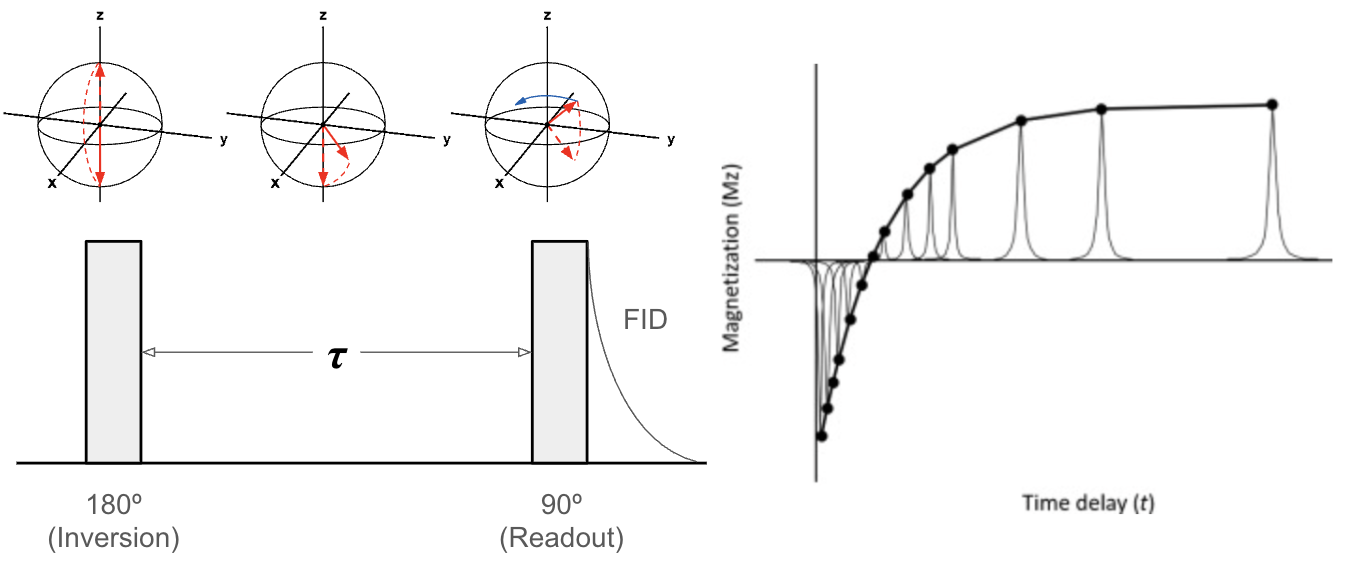
\includegraphics[width=0.8\textwidth]{figures/inv-rec-sequence.png}
    \caption{The inversion recovery pulse sequence, overlaid with the corresponding magnetization response. A 180º RF pulse rotates the magnetization so that the spins are anti-parallel to the static magnetic field. For a time $\tau$, the magnetization is allowed to recover to its equilibrium state. The resulting state is then rotated 90º, inducing a FID response due to its precession about the static field's axis (blue arrow). The maximum FID amplitude is recorded for several values of $\tau$, leading to the inversion recovery curve on the right.}
    \label{fig:inv-rec-seq}
\end{figure*}

This defines the expected inversion recovery curve from Figure~\ref{fig:inv-rec-seq}. In Section~\ref{sec:experiment}, we explore how the measurement apparatus further modifies the inversion recovery model.

After this delay, a $\tfrac{\pi}{2}$ pulse is applied to rotate the longitudinal magnetization into the transverse plane, where it can be detected. Repeating this procedure for different values of $\tau$ yields a recovery curve, from which $T_1$ can be extracted. The longitudinal magnetization evolves according to Eq.~\ref{eq:T1_recovery}, allowing $T_1$ to be extracted from the recovery curve.

\subsection{The Ornstein-Uhlenbeck model}
\label{sec:ou_model}

\subsubsection{Assumptions on stochastic field fluctuations}
\label{sec:assumptions}
Experimentally, the magnetic field experienced by each spin is not perfectly static, but fluctuates due to molecular motion and interactions with neighboring spins. These fluctuations introduce randomness into the spin dynamics, leading to both dephasing and energy exchange. Modeling these fluctuations as a stochastic process provides a direct link between microscopic dynamics and the observed relaxation times $T_1$ and $T_2$.

In modeling the fluctuating local magnetic fields experienced by nuclear spins, we assume that the sample is in thermal equilibrium and that it is weakly coupled to the macroscopic environment, implying that the statistical properties of the local fields do not change in time. The local field $\mathfrak{B} (t)$ at a given nucleus can thus be expressed as the sum of several, smaller contributions from other nuclei:
\begin{equation}
    \mathfrak{B}(t) = \sum_i b_i (t).
    \label{eq:sum_of_parts}
\end{equation}
Under moderate temperatures and viscosities, and at sufficiently low spin densities, the field fluctuations decorrelate on timescales much shorter than the overall relaxation dynamics. This justifies a Markov (memoryless) approximation. Furthermore, we assume only small deviations between the local field and its mean value, so that their relaxation occurs linearly and is characterized by a single correlation time $\tau_c$.

Finally, Eq.~\ref{eq:sum_of_parts} suggests that the total field $B$ may be expressed as the sum of many weakly-correlated/independent weak field sources. Therefore, a central-limit-type argument implies that the distribution of the total field approaches a Gaussian, regardless of the detailed statistics of the individual contributions.

\subsubsection{Stochastic Differential Equations and the Ornstein–Uhlenbeck Model}
\label{sec:SDEtoOU}
We begin by considering a deterministic model for relaxation toward equilibrium. Let an observable $X_t \equiv X(t)$ obey the following linear relaxation law
\begin{equation}
    \frac{dX_t}{dt} = -\theta X_t
    \label{eq:deterministic}
\end{equation}
for some constant $\theta>0$. The equation above admits solutions of the form $X_t = X_0 e^{-\theta t}$, describing exponential decay with characteristic time $\theta^{-1}$. One may immediately notice similarity with Eqs.~\ref{eq:T1_recovery} and~\ref{eq:T2_recovery}, and might suggest that Eq.~\ref{eq:deterministic} is sufficient for modeling microscopic observables $X_t$.

However, deterministic equations cannot fully capture the effect of rapidly fluctuating microscopic fields, which appear random at the level of a single spin. We therefore seek to incorporate stochastic fluctuations into Eq.~\ref{eq:deterministic} by introducing a noise term:
\begin{equation*}
    \frac{dX_t}{dt} = -\theta X_t + \mathrm{noise}
\end{equation*}
The term `noise' here is only heuristic, as rapid fluctuations are too irregular to be represented as an ordinary differentiable function of time. In stochastic calculus, such fluctuations are modeled by Gaussian white noise, also known as a \textit{Wiener process} $W_t$, where the increment $dW_t$ in the time interval $dt$ is normally distributed; that is, $dW_t\sim\mathcal{N}(0,dt)$.

The stochastic contribution is thus expressed in terms of $dW_t$, yielding the stochastic differential equation
\begin{equation*}
    dX_t =
    \underbrace{-\theta X_t\, dt}_{\text{deterministic}}
    +
    \underbrace{\sigma\, dW_t}_{\text{stochastic}}
\end{equation*}
where $\sigma$ denotes the fluctuation amplitude. 

The assumptions outlined in Sec.~\ref{sec:assumptions} strongly constrain the form of the stochastic model. Specifically, the Markov approximation implies that the dynamics of the local field must be memoryless, while the Gaussianity of fluctuations suggests that the noise term should be driven by a Wiener process. Furthermore, the assumption of small deviations from equilibrium justifies a linear restoring term (the deterministic part of the previous equation). Together, these considerations uniquely lead to a mean-reverting linear stochastic differential equation, namely the Ornstein--Uhlenbeck process.

If we take the observable $X_t$ to represent the local magnetic field $\mathfrak{B}_t$ experienced by a spin, the above equation becomes
\begin{equation}
    d\mathfrak{B}_t = -\frac{1}{\tau_c} \mathfrak{B}_t dt + \sigma dW_t,
    \label{eq:OUsde}
\end{equation}
where we identify $\theta = \tau_c^{-1}$ as the inverse correlation time of local field fluctuations.

The solution to Eq.~\ref{eq:OUsde} can be found by multiplying both sides of the equation by an integrating factor $e^{at}$ and using the identity $d\left(e^{at}\mathfrak{B}_t\right)=\sigma e^{at}dW_t$, yielding
\begin{equation}
    \mathfrak{B}_t = \mathfrak{B}_0 e^{-t/\tau_c}
    + \sigma \int_0^t e^{-(t-s)/\tau_c}\, dW_s.
    \label{eq:OU_soln}
\end{equation}
Let $s = t + T$ for some $T>0$. In the long-time (stationary) regime where the influence of the initial condition has decayed, one finds the two-time autocorrelation function
\begin{equation}
    C(T) = \langle \mathfrak{B}(t)\mathfrak{B}(t+T)\rangle = \frac{\sigma^2\tau_c}{2}\,e^{-|T|/\tau_c},
    \label{eq:autocorr}
\end{equation}
where $\lim_{t\rightarrow\infty}\mathrm{Var}\,\mathfrak{B}_t=\sigma^2\tau_c/2$. The field fluctuations therefore exhibit exponential memory decay with characteristic correlation time $\tau_c$.

Now, the longitudinal relaxation $T_1$ is driven by the transverse fluctuating fields at the Larmor frequency $\omega_0$, and $T_2$ receives contributions from all components of the local field. We further simplify the model by assuming that the fluctuations $\boldsymbol{\mathfrak{B}}_t = \left(\mathfrak{B}_x(t),\mathfrak{B}_y(t),\mathfrak{B}_z(t)\right)$ are isotropic and uncorrelated between components:
\begin{equation*}
    \langle \mathfrak{B}_i (t)\mathfrak{B}_j (t+T)\rangle
    =
    \delta_{ij}\,C(T),
    \qquad C(0)=\Delta^2.
\end{equation*}
where $\Delta^2 = \sigma^2\tau_c / 2$.

Defining the spectral density through an application of the Wiener-Khinchin theorem,
\begin{equation*}
    J(\omega)
    =
    \int_{-\infty}^{\infty} C(t)e^{-i\omega t}\,dt,
\end{equation*}
the relaxation rates are given by \cite{slichter1990principles}
\begin{align}
    \frac{1}{T_1} &= \gamma^2 \big[ J_x(\omega_0) + J_y(\omega_0) \big], \notag \\
    \frac{1}{T_2} &= \frac{1}{2T_1} + \gamma^2 J_z(0).
    \label{eq:T2_dephasing_energy}
\end{align}
Under isotropy, $J_x = J_y = J_z = J$, so that
\begin{align*}
    \frac{1}{T_1} &= 2\gamma^2 J(\omega_0), \\
    \frac{1}{T_2} &= \gamma^2 J(0) + \gamma^2 J(\omega_0).
\end{align*}
The OU spectral density is given by calculating the Fourier transform of the correlation function in Eq.~\ref{eq:autocorr}. Substituting it into the equations above, we obtain
\begin{align*}
    \frac{1}{T_1}
    &=
    \frac{4\gamma^2 \Delta^2 \tau_c}{1+\omega_0^2 \tau_c^2}, \\
    \frac{1}{T_2}
    &=
    2\gamma^2 \Delta^2 \tau_c
    +
    \frac{2\gamma^2 \Delta^2 \tau_c}{1+\omega_0^2 \tau_c^2}.
\end{align*}

These expressions establish a one-to-one mapping between the relaxation parameters $\left(T_1, T_2\right)$ and the OU parameters $(\tau_c, \Delta)$ given $T_1 > T_2$, enabling direct inference of microscopic fluctuation dynamics from macroscopic observables. Eliminating $\Delta$ gives an expression for $\tau_c$:
\begin{equation}
    \tau_c
    =
    \frac{1}{\omega_0}
    \sqrt{2\left(\frac{T_1}{T_2} - 1\right)}.
    \label{eq:tau_c}
\end{equation}
Once $\tau_c$ is determined, the fluctuation amplitude follows from
\begin{equation}
    \Delta^2
    =
    \frac{1}{4\gamma^2 \tau_c T_1}
    \left(1+\omega_0^2 \tau_c^2\right).
    \label{eq:delta_sq}
\end{equation}

\subsection{Stochastic simulation of NMR signals}
\label{sec:simulation}
To assess the validity of the OU model, we simulate pulsed NMR signals using the inferred parameters $\left(\tau_c,\Delta\right)$ and compare the resulting spin echo decay to that obtained experimentally. Each component $\mathfrak{B}_i (t)$ of the local field obeys the OU stochastic differential equation (Eq.~\ref{eq:OUsde}). On a discrete time interval $t\rightarrow t+\delta t$, Eq.~\ref{eq:OU_soln} reads
\begin{equation*}
    \mathfrak{B}_{t+\delta t} = \mathfrak{B}_0 e^{-\delta t/\tau_c}
    + \sigma \int_t^{t+\delta t} e^{-(t+\delta t-s)/\tau_c}\, dW_s,
\end{equation*}
from which we derive the update rule for the numerical simulation,
\begin{equation*}
    \mathfrak{B}_{t+\delta t} = \mathfrak{B}_t e^{-\delta t/\tau_c} + \sqrt{\Delta^2\left(1-e^{-2\delta t/\tau_c}\right)}\xi,
\end{equation*}
where $\xi \sim \mathcal{N}\left(0,1\right)$.

Since the observable of interest is governed by phase coherence, we model the stochastic phase accumulation induced by longitudinal field fluctuations, rather than solving the full Bloch equations.

In pulsed NMR, the spins are (ideally) aligned with the transverse plane after a $\tfrac{\pi}{2}$ pulse. The $k$th spin thus precesses around the static field $\mathbf{B}$. In reality, each spin experiences a time-dependent local field, so its instantaneous precession frequency is
\begin{equation*}
    \omega_k (t) = \gamma\left(B_0 + \mathfrak{B}_z^{(k)}(t)\right) = \omega_0 + \delta\omega_k (t)
\end{equation*}
Here, only the longitudinal component $\mathfrak{B}_z^{(k)}(t)$ contributes to frequency shifts, and hence a stochastic phase accumulation $\delta\omega_k (t) = \gamma\mathfrak{B}_z^{(k)}(t)$.

The phase of a single spin is given by the time integral of its frequency. In the rotating frame, the $\omega_0$ term vanishes, so that
\begin{equation*}
    \phi_k (t) = \gamma\int_{0}^t \mathfrak{B}_z^{(k)}(t^\prime)\,dt^{\prime},
\end{equation*}
where we introduce a dummy variable $t^\prime$. Now, the NMR signal $S(t)$ comprises the sum of all spins, so we may express it as an \textit{ensemble average} over stochastic realizations:
\begin{equation}
    S(t) = \left\langle e^{-i\phi (t)}\right\rangle
    \label{eq:simulated_signal}
\end{equation}
where
\begin{equation}
    \phi (t) = \gamma\int_{0}^t \mathfrak{B}_z (t^\prime)\,dt^{\prime},
    \label{eq:stochastic_phase}
\end{equation}

For the spin-echo sequence, we treat the RF pulses as instantaneous rotations. This approximation is justified because the pulse duration $t_p$ is short compared to the timescale of stochastic dephasing, so that negligible phase is accumulated during the pulses themselves. The stochastic phase accumulation may therefore be written piecewise, with the $\pi$ pulse reversing the sign of the subsequent phase evolution. Hence, for a pulse sequence of duration $2\tau$, we have
\begin{equation}
    \phi_{\text{echo}}(2\tau) = \gamma\left(\int_0^{\tau}\mathfrak{B}_z (t)\,dt - \int_\tau^{2\tau}\mathfrak{B}_z(t)\,dt\right)
    \label{eq:echo_phase}
\end{equation}

As such, we assume that the accumulated phase from Eq.~\ref{eq:stochastic_phase} remains a Gaussian random variable. This is justified when the stochastic field is weak and rapidly fluctuating so that by Eq.~\ref{eq:sum_of_parts} the phase results from the sum of many small, independent contributions. By the central limit theorem, the phase distribution approaches a normal distribution mean zero and variance $\mathrm{Var\,}\phi (t) = \left\langle \phi^2 (t)\right\rangle$, thereby yielding
\begin{equation*}
    \left\langle e^{i\phi(t)} \right\rangle = e^{-\frac{1}{2} \left\langle \phi^2 (t)\right\rangle}.
\end{equation*}
For the OU model, the phase variance is determined entirely by the autocorrelation in Eq.~\ref{eq:autocorr}:
\begin{align*}
    \left\langle\phi^2(t)\right\rangle &= \gamma^2 \int_0^t \int_0^t \left\langle \mathfrak{B}_z (t_1) \mathfrak{B}_z (t_2)\right\rangle\,dt_1dt_2\\
    &\propto\begin{cases}
            t^2,&\quad t\ll \tau_c\\
            t,&\quad t\gg\tau_c
        \end{cases}.
\end{align*}
In other words, the ensemble-averaged signal $S(t)$ will emulate the transverse magnetization's exponential decay, provided the field's correlation time is much shorter than the total observation time. This captures the spin-echo envelope directly, while avoiding unnecessary complication from pulse dynamics.

\section{Experiment}
\label{sec:experiment}

\subsection{Initial experimental considerations}
\label{sec:considerations}

\subsubsection{Sample selection and physical motivation}
\label{sec:samples}
To probe the validity of the OU model in different regimes, we extract the parameters $(T_1,T_2)$ for light and heavy mineral oil. These samples are chosen as examples of fast and slow molecular dynamics, respectively. Light mineral oil is less dense, and is expected to exhibit relatively fast, weakly correlated molecular motion. This implies that magnetic interactions between any two spins are short-lived, thus producing low-amplitude, rapidly fluctuating local magnetic fields with short correlation times. In this regime, the assumptions underlying the OU model -- namely Gaussian statistics and short memory -- are expected to hold, making it an appropriate candidate for model validation. On the other hand, heavy oil is denser and consists of larger, more complex molecules with additional modes of interaction, leading to slower dynamics and longer correlation times and larger field amplitudes.

Ideally, a simple liquid such as distilled water or ethanol would provide a more direct validation of the OU model, as these systems are well-approximated by rapid fluctuating, weakly correlated molecular environments. However, in practice, obtaining reliable measurements of $(T_1, T_2)$ for these samples proved challenging within the constraints of the present apparatus. In particular, the relatively long relaxation times, sensitivity to experimental conditions (e.g., tuning conditions and repetition timing), and low proton density \cite{teachspin_ps2} led to significant variability in the measured signals. As a result, light mineral oil was adopted as a practical validation sample, providing a balance between sufficiently fast dynamics and experimental robustness.

\subsubsection{Measurement and signal interpretation}
\label{sec:signal}
The TeachSpin™ Pulsed/CW NMR apparatus consists of three primary components: a permanent magnet assembly with an integrated sample coil, the PS2 receiver module, and the PS2 controller. The sample coil, positioned within the uniform magnetic field produced by the Neodymium-Iron-Boron magnets, generates the transverse radio-frequency field used to manipulate the nuclear magnetization. The response from the sample involves a changing magnetic field, which in turn induces a current in the sample coil. The resulting voltage is then output via an envelope channel on the PS2 receiver module, which can then be visualized on an oscilloscope. 

In particular, the envelope detection channel outputs a signal proportional to the \textit{magnitude} of the transverse magnetization. As such, the model for the inversion recovery must be adjusted to fit the observed signal. A careful observation of Eq.~\ref{eq:inv-rec-eq} reveals that a crude estimate of $T_1$ could be obtained by determining the time $\tau_0$ in between pulses for which the magnetization response is zero; that is, setting $2\exp(-\tau/T_1)=1$, we have
\begin{equation*}
    \tau_0 = \frac{T_1}{\ln{2}}.
\end{equation*}
However, under an absolute-valued envelope, there is no such zero-crossing. Instead, $\tau_0$ defines the location of the cusp on the following curve:
\begin{equation}
    S(\tau) = A\left\lvert 1-2e^{-\tau/T_1}\right\rvert + C,
    \label{eq:inv-rec-model}
\end{equation}
where $A$ and $C$ are fitting constants.

Naturally, this is not a problem for the spin-echo measurements, where the absolute value does not change the form of Eq.~\ref{eq:T2_recovery}. As such, the equation used to fit the data is
\begin{equation}
    S(2\tau) = Ae^{-2\tau/T_2} + C,
    \label{eq:spin-echo-model}
\end{equation}
with $A$ and $C$ serving the same purpose. However, when comparing the raw data with the signal extracted from Eq.~\ref{eq:simulated_signal}, the offset $C$ is expected to produce normalization artifacts that detract from the OU model validation.

\subsubsection{Apparatus tuning and experimental stability}
\label{sec:tuning}
Accurate measurement of relaxation times requires careful tuning of the NMR apparatus. In particular, the resonant frequency of the probe must be matched to the Larmor frequency (approximately 21 MHz for protons in the present setup), and the impedance of the sample coil must be properly adjusted to maximize signal transfer to the receiver. Small deviations in tuning can significantly reduce the amplitude and stability of the observed signal, directly impacting the reliability of extracted relaxation parameters.

To ensure a correct application of pulses in the inversion recovery and spin echo pulse sequences, the PS2 module's receiver frequency was tuned to achieve a maximum FID amplitude and the lowest-amplitude/fastest-decaying beats. In addition, to minimize the effect of field inhomogeneities, the PS2 controller's magnetic field gradient dials were adjusted to achieve the longest possible decay time, shown in Figure~\ref{fig:FID-tuning}. We note, however, that there may be more than one combination of field gradients that generates the same FID decay time, and that slight miscalibrations in this regard may affect the fidelity of the spin echo response.
\begin{figure}[t]
    \centering
    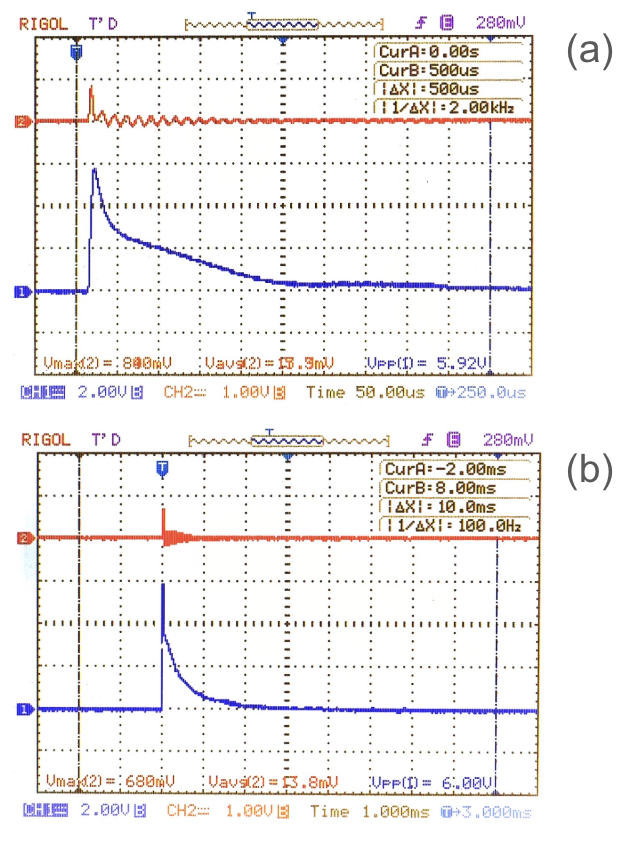
\includegraphics[width=0.7\linewidth]{figures/FID-tuning.png}
    \caption{Adjusting the FID (blue) for maximum decay time; (a) shows the FID response before adjusting magnetic field gradients, where one observes a decay time on the order of a few hundred microseconds as dictated by the time-division scale on the bottom right corner (`Time 50.00 µs'); (b) shows the FID response after adjusting the field gradients, noting a decay visible over a few milliseconds -- an order of magnitude longer than the previous set up.}
    \label{fig:FID-tuning}
\end{figure}

Additional sources of instability arise from pulse calibration and repetition timing. The FID amplitude is also used to calibrate the pulse lengths, with the largest amplitude corresponding to a correctly calibrated $\tfrac{\pi}{2}$ pulse, and minimum amplitude corresponding to a $\pi$ pulse. It is easier to tune the pulse length to achieve the least possible FID amplitude, and divide that result by two for the $\tfrac{\pi}{2}$ pulse. As such, slightly miscalibrated pulse lengths lead to  deviations from ideal flip angles, resulting in incomplete excitation or refocusing and thereby affecting both inversion recovery and spin-echo measurements. Furthermore, insufficient repetition delay between pulse sequences can prevent full recovery of the longitudinal magnetization, leading to systematic underestimation of NMR parameters.

Additionally, temporal fluctuations in signal amplitude were observed even under nominally fixed conditions, likely due to a combination of electronic noise, drift in tuning, and environmental perturbations. These effects limit the precision of individual measurements and motivate the use of repeated trials and curve fitting to extract reliable relaxation times.

\subsection{Extraction of NMR parameters}
\label{sec:nmr_expr}

\subsubsection{Extraction of $T_1$: inversion recovery}
\label{sec:T1-recovery}
The inversion recovery sequence inverts the equilibrium magnetization to its negative value, allows the system to relax toward equilibrium over a time $\tau$, then converts $M_z(\tau)$ to a measurable signal via a $\tfrac{\pi}{2}$ readout pulse. We vary $\tau$ so as to capture both sides of the zero crossing of Eq.~\ref{eq:inv-rec-eq}, allowing an estimate of the cusp $\tau_0$ of Eq.~\ref{eq:inv-rec-model}. We further ensure that the pulse sequence repetition rate allows for full magnetization recovery in between pulse sequences. The maximum amplitude of the FID resulting from the readout pulse (pulse B) is recorded for each value of $\tau$ except at the cusp, where the signal is dominated by electronic noise. Figure~\ref{fig:T1_curves} demonstrates the inversion recovery curves modified under Eq.~\ref{eq:inv-rec-model}.
\begin{figure}[t]
    \centering
    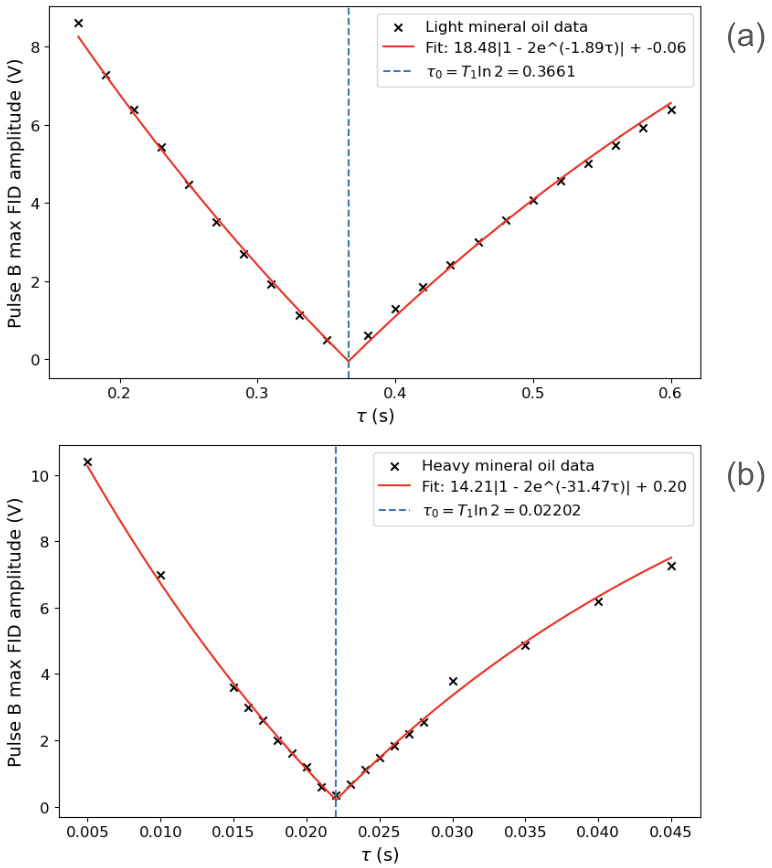
\includegraphics[width=\linewidth]{figures/T1_results.png}
    \caption{Inversion recovery measurements used to extract the longitudinal relaxation time $T_1$ for (a) light mineral oil and (b) heavy mineral oil. The measured signal corresponds to the envelope-detected amplitude following the $\tfrac{\pi}{2}$ readout pulse and is plotted as a function of the delay time $\tau$. The data are fit to the model $S(\tau) = A\left\lvert 1-2e^{-\tau/T_1}\right\rvert + C$, accounting for the magnitude-only detection of the receiver. The characteristic cusp at $\tau_0=T_1\ln{2}$ (dashed line) marks the zero-crossing of the underlying longitudinal magnetization. The extracted values of $T_1$ differ significantly between the two samples, reflecting distinct dynamical regimes that are later used to infer stochastic field parameters.}
    \label{fig:T1_curves}
\end{figure}

While $T_1$ and its associated uncertainty can be inferred from the nonlinear least-squares fit, it is useful to compare it against the estimate provided by $\tau_0$, which we denote $\tilde{T}_1$. From the cusp locations, we obtain preliminary estimates $\tilde{T}_{1,l}\approx 528\,\mathrm{ms}$ for light mineral oil and $\tilde{T}_{1,h}\approx 31.8\,\mathrm{ms}$ for heavy mineral oil. Indeed, these agree closely with the fitted values in Figure~\ref{fig:T1_curves}:
\begin{equation*}
    T_{1,l} = 528\pm 1\,\mathrm{ms} \qquad T_{1,h}= 31.8\pm 0.1 \,\mathrm{ms}.
\end{equation*}
The substantial difference between these relaxation times reflects distinct dynamical regimes in the two samples. In light mineral oil, the longer $T_1$ indicates weaker coupling between the nuclear spins and their environment, consistent with rapid local field fluctuations that are inefficient at driving transitions at the Larmor frequency. In contrast, the shorter $T_1$ observed in heavy mineral oil indicates more efficient energy exchange with the lattice, arising from slower, more strongly correlated fluctuations in the local magnetic environment.

\subsubsection{Extracting $T_2$: spin echo}
\label{sec:T2-echo}
To determine the spin-spin relaxation time $T_2$, we employ the spin echo sequence described in Section~\ref{sec:pnmr}, sweeping over values of $\tau$ to obtain the spin echo decay curves for each sample (Figure~\ref{fig:T2_curves}). The $\tau$ values in the sweep are chosen so that there is no overlap with the initial FID envelope, and the maximum echo height is measured using a cursor on a RIGOL oscilloscope, with the bottom reference set to zero. As in the previous section, we ensure full magnetization recovery by setting the pulse sequence repetition delay to several times the value of $T_1$.
\begin{figure}[!t]
    \centering
    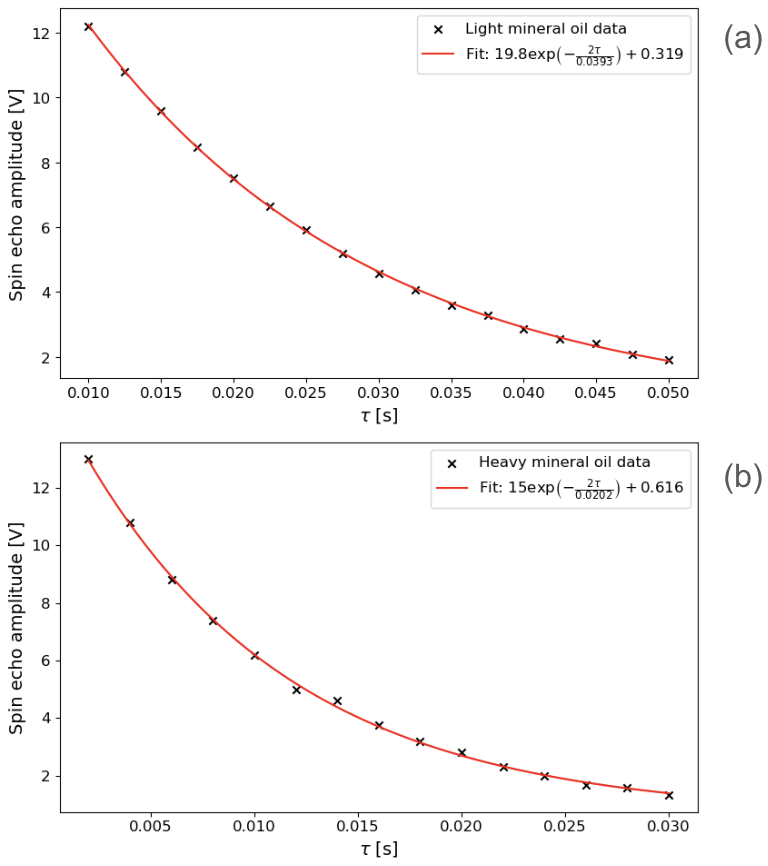
\includegraphics[width=\linewidth]{figures/T2_results.png}
    \caption{Spin-echo measurements used to extract the transverse relaxation time $T_2$ for (a) light mineral oil and (b) heavy mineral oil. The plotted signal corresponds to the envelope-detected peak amplitude of the spin echo as a function of the delay time $\tau$ in the $\tfrac{\pi}{2}\,-\,\tau\,-\,\pi\,-\,\tau$ sequence. The data are fit to the nonlinear least-squares model $S(2\tau) = Ae^{-2\tau/T_2} + C$. The extracted $T_2$ values show a clear reduction of coherence time for heavy mineral oil relative to light mineral oil, consistent with stronger and more slowly varying local field fluctuations in the former.}
    \label{fig:T2_curves}
\end{figure}

The spin echo measurements show clear exponential decays for both samples, allowing $T_2$ to be reliably extracted from model of Eq.~\ref{eq:spin-echo-model}. The data predict
\begin{equation*}
    T_{2,l} = 39.3\pm 0.5\,\mathrm{ms} \qquad T_{2,h} = 20.2\pm 0.5\,\mathrm{ms}
\end{equation*}
for light and heavy mineral oil, respectively. The heavy mineral oil loses transverse coherence roughly twice as quickly as the light mineral oil, consistent with stronger local field fluctuations and less effective motional averaging in the heavier sample. 

Unlike the inversion recovery measurement, the spin-echo sequence suppresses dephasing due to static field inhomogeneity. Therefore, the observed decay of the echo peak is primarily associated with irreversible loss of transverse coherence. However, the measured $T_2$ is not purely a dephasing time; it contains also an energy relaxation contribution $1/2T_1$, as seen in Eq.~\ref{eq:T2_dephasing_energy}. Since $T_{1,h} \ll T_{1,l}$, energy relaxation contributes more strongly to the transverse decay in heavy mineral oil. This means that $T_{2,h} < T_{2,l}$ reflects both enhanced stochastic dephasing and faster spin-lattice relaxation.
\begin{table}[t]
    \centering
    \begin{tabular}{l c c}
        \hline
        \textbf{Sample} & \boldmath{$T_1$ (ms)} & \boldmath{$T_2$ (ms)} \\
        \hline
        Light mineral oil & $528 \pm 1$ & $39.3 \pm 0.5$ \\
        Heavy mineral oil & $31.8 \pm 0.1$ & $20.2 \pm 0.5$ \\
        \hline
    \end{tabular}
    \caption{Measured longitudinal ($T_1$) and transverse ($T_2$) relaxation times for light and heavy mineral oil.}
    \label{tab:relaxation_times}
\end{table}
\begin{table}[t]
    \centering
    \begin{tabular}{lccc}
        \hline
        \textbf{Sample} & \boldmath{$\tau_c$ (ns)} & $\boldsymbol{\Delta^2}\,(\mathrm{G}^2)$ & $\boldsymbol{\sigma}\,(\mathrm{T}\cdot\mathrm{s}^{-1/2})$ \\
        \hline
        Light Oil & 37.6 & 0.45 & 0.49 \\
        Heavy Oil & 8.09 & 2.91 & 2.68 \\
        \hline
    \end{tabular}
    \caption{OU parameters $(\tau_c, \Delta^2, \sigma)$ inferred from the relaxation parameters in Table~\ref{tab:relaxation_times}. Note that $\Delta^2$ is proportional to $\sigma^2$ through $\tau_c/2$.}
    \label{tab:OU_params}
\end{table}

A summary of the results for the experimental section is found in Table~\ref{tab:relaxation_times}. The extracted NMR parameters $(T_1,T_2)_l$ for light mineral oil and $(T_1,T_2)_h$ for heavy mineral oil provide the main experimental benchmark for the OU phase-accumulation simulation.

\subsection{Simulation results}
\label{sec:simulation_results}

\subsubsection{Ornstein-Uhlenbeck parameters}
\label{sec:OU_params}
We now map the experimentally measured relaxation times into the Ornstein--Uhlenbeck (OU) parameters $(\tau_c,\Delta^2)$ using Eqs.~\ref{eq:tau_c} and~\ref{eq:delta_sq}, with the results summarized in Table~\ref{tab:OU_params}. 

Notably, the inferred correlation time for light mineral oil, $\tau_{c,l} = 37.6\,\mathrm{ns}$, is larger than that of heavy mineral oil, $\tau_{c,h} = 8.09\,\mathrm{ns}$. This appears counterintuitive: one might expect the lighter sample, which exhibits more rapid molecular motion, to correspond to a shorter correlation time. However, the extracted values must be interpreted in the context of the relaxation relations used to infer them.

From Eq.~\ref{eq:tau_c}, the correlation time is determined by the ratio $T_1/T_2$. For heavy mineral oil, $T_{1,h}/T_{2,h} \approx 3/2$, which places the system near the intermediate regime $\omega_0 \tau_{c,h} \sim 1$, consistent with fluctuations occurring on timescales comparable to the Larmor period. In contrast, for light mineral oil, $T_{1,l}/T_{2,l} \approx 13$, which yields $\omega_0 \tau_{c,l} \gg 1$. Within the OU framework, this corresponds to a slow-fluctuation regime, where the local field evolves on timescales longer than the spin precession period. A possible conclusion from this result is that he assumption of isotropic fluctuations is not valid for light oil, because $T_{1,l}$ and $T_{2,l}$ imply an unphysical or counterintuitive OU correlation time when forced into a single isotropic noise model. In particular, $T_{2,l} \ll T_{1,l}$ suggests that transverse coherence is being lost through extraneous dephasing mechanisms.

This highlights an important limitation of the model: the inferred OU parameters are not direct measurements of microscopic dynamics, but rather effective quantities constrained by the measured relaxation times under the assumptions of isotropic, memoriless fluctuations. As a result, this apparent slow-fluctuation regime for light mineral oil is not a direct physical measurement, but rather a consequence of fitting the data to an inadequate single-timescale model.

\subsubsection{Comparison of simulated and experimental spin echo decay}
\label{sec:comparison}
We now simulate the stochastic phase accumulation for the spin echo sequence (Eq.~\ref{eq:echo_phase}) and compare it to the experimental signal captured in Figure~\ref{fig:T2_curves}. In light of the effect of energy relaxation on the inferred OU parameters, we include a correction to the decay envelope for further comparison (denoted by the dashed lines titled `corrected' in Figure~\ref{fig:final}). 
\begin{figure*}[t]
    \centering
    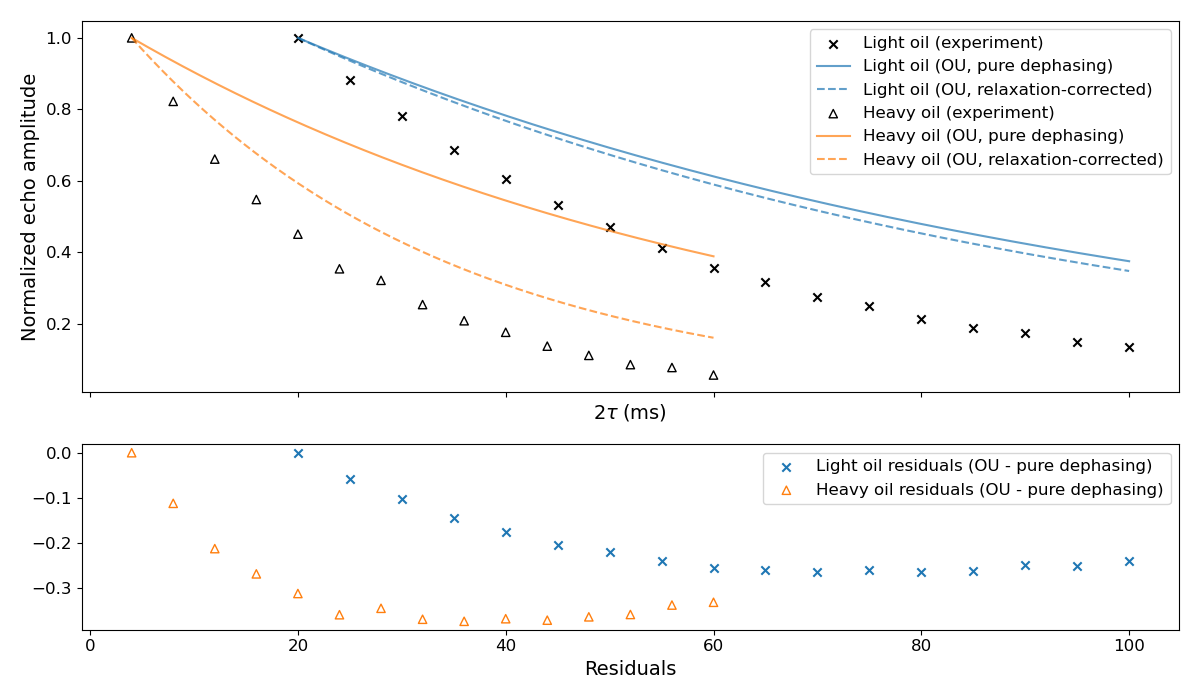
\includegraphics[width=0.8\textwidth]{figures/OU_vs_exp.png}
    \caption{A plot of the normalized spin echo decay curve, including the simulated signal accounting for only pure dephasing (solid lines) and for energy relaxation corrections (dashed lines), as well as residuals between experimental and simulated signals for the pure dephasing simulation. While the relaxation-corrected model improves agreement with experiment, deviations remain indicating the presence of dephasing mechanisms not captured by the isotropic OU approximation. In particular, the correction for light mineral oil is almost negligible, since the large observed $T_{1,l}$ makes the first term in Eq.~\ref{eq:dephasing_plus_relaxation} negligible.}
    \label{fig:final}
\end{figure*}

Energy relaxation drives changes in the population of each spin state: $\left\lvert\uparrow\right\rangle$ for $m_I = +\tfrac{1}{2}$ and $\left\lvert\downarrow\right\rangle$ for $m_I = -\tfrac{1}{2}$. In the $\{\left\lvert\uparrow\right\rangle ,\left\lvert\downarrow\right\rangle\}$ basis, the density matrix for a spin-$\tfrac{1}{2}$ system is
\begin{equation*}
    \rho = \begin{pmatrix}
        \rho_{\uparrow\uparrow} & \rho_{\uparrow\downarrow}\\
        \rho_{\downarrow\uparrow} & \rho_{\downarrow\downarrow}
    \end{pmatrix},
\end{equation*}
where the diagonal elements determine longitudinal magnetization, and the off-diagonal elements determine transverse magnetization. Since spin flips do not preserve the phase of the original state, phase coherence is destroyed \cite{Levitt2008}, and
\begin{equation*}
    \rho_{\uparrow\downarrow} (t) \sim e^{-t/2T_1}.
\end{equation*}
Meanwhile, pure dephasing does not affect the diagonal populations, but randomizes the relative phase between $\left\lvert\uparrow\right\rangle$ and $\left\lvert\downarrow\right\rangle$, giving
\begin{equation*}
    \rho_{\uparrow\downarrow} (t) \sim e^{-t/T_{\phi}},
\end{equation*}
where $T_{\phi}$ is the pure dephasing time. Assuming these two processes are independent, we have
\begin{equation*}
    \rho_{\uparrow\downarrow} (t) = \rho_{\uparrow\downarrow} (0) \exp{\left[-t\left(\frac{1}{2T_1} + \frac{1}{T_{\phi}}\right)\right]},
\end{equation*}
proportional to the transverse magnetization. But if $M_{xy}=M_0\exp{-t/T_2}$, then
\begin{equation}
    \frac{1}{T_2} = \frac{1}{2T_1} + \frac{1}{T_{\phi}}.
    \label{eq:dephasing_plus_relaxation}
\end{equation}
This is directly identifiable with Eq.~\ref{eq:T2_dephasing_energy}. As such, we modify Eq.~\ref{eq:simulated_signal} to include the relaxation correction as follows:
\begin{equation*}
    S(2\tau) = \left\langle e^{-i\phi_{\text{echo}} (2\tau)}\right\rangle e^{-\tau/T_1}
\end{equation*}

The comparison between experimental spin-echo decay and OU-based simulations reveals sample-dependent systematic discrepancies. For both light and heavy mineral oil, the pure dephasing model based on stochastic phase accumulation overestimates the coherence, as evidenced by the consistently negative residuals. Although the model qualitatively captures it, the longitudinal field fluctuations alone are evidently insufficient to account for the observed transverse decay.

Incorporating the contribution of energy relaxation through an additional exponential factor improves agreement with experiment, particularly for heavy mineral oil, where $T_{1,h}$ is small and contributes significantly to Eq.~\ref{eq:dephasing_plus_relaxation}. In this case, the corrected model provides a better overall signal decay rate, suggesting that the combined effects of dephasing and relaxation are reasonably well described by a single-timescale OU process. This is consistent with the inferred regime $\omega_0 \tau_c \sim 1$, where fluctuations occur on timescales similar to the Larmor period.

In contrast, the light oil data exhibit persistent deviations even after the inclusion of the relaxation correction. The relatively long $T_1$ implies that energy relaxation contributes only weakly to the transverse decay, so the observed discrepancy must arise from additional dephasing mechanisms. One possible contribution is molecular diffusion in the presence of residual magnetic field gradients not eliminated in the initial tuning process, which scale like $\exp{(-\tau^3)}$ \cite{teachspin_ps2}. In this case, diffusive motion causes spins to sample spatial variations in the local field, leading to an additional, effectively irreversible phase dispersion that is not rectified by the spin-echo sequence. This mechanism plays a larger role in the light mineral oil sample due to its reduced density and constituents' molecular size, yet is not captured by the OU model, which assumes a spatially homogeneous stochastic field.

Taken together, these results indicate that while the OU model provides a self-consistent description of the heavy oil data, it fails to capture the full relaxation behavior of light mineral oil. This highlights a key limitation of the model: the assumption that all field components can be described by a single isotropic stochastic process is not universally valid across different dynamical regimes.

\section{Conclusion}
\label{sec:conclusion}
In this work, we investigated nuclear spin relaxation in liquid samples using pulsed NMR and evaluated the applicability of an Ornstein--Uhlenbeck (OU) stochastic model for describing transverse dephasing. By measuring the longitudinal and transverse relaxation times, $T_1$ and $T_2$, via inversion recovery and spin-echo experiments, we inferred effective OU parameters and used them to simulate stochastic phase accumulation.

Comparison between simulation and experiment revealed that a pure dephasing model based on longitudinal field fluctuations alone systematically overestimates the coherence for both samples. Incorporating the contribution of energy relaxation through Eq.~\ref{eq:dephasing_plus_relaxation} improves agreement, particularly for heavy mineral oil, where the model provides a reasonably self-consistent description of the observed dynamics. In contrast, light mineral oil exhibits significant deviations even after accounting for relaxation effects. The large ratio $T_1/T_2$ indicates that transverse coherence is dominated by dephasing mechanisms not captured by the isotropic OU model. Possible contributions include molecular diffusion in the presence of residual magnetic field gradients, multi-timescale decorrelation warranted by the multiple motional processes that occur inside a liquid, and non-Markovian fluctuations, all of which violate the assumption of a single, spatially homogeneous stochastic process.

These results highlight both the utility and the limitations of the OU framework. While it provides a tractable and physically interpretable model for relaxation in certain regimes, its underlying assumptions are not universally valid across different dynamical environments.

\bibliographystyle{unsrt}
\bibliography{report}% Produces the bibliography via BibTeX.

\end{document}
%
% ****** End of file apssamp.tex ******